\newpage
%%%%%%%%%%%%%%%%%%%%%%%%%%%%----->SECCIÓN 2<-----%%%%%%%%%%%%%%%%%%%%%%%%%
\chapter{Rayos cósmicos}
%%%%%%%%%%%%%%%%%% NEWWWW
Los rayos cósmicos (CR) son partículas cargadas que viajan a través del espacio intergaláctico a velocidades cercanas a la luz. Estas partículas que provienen de diversas fuentes, incluyendo el Sol, supernovas, pulsares, agujeros negros entre otras, son en su mayoría protones y núcleos atómicos. Su composición es diversa, con una predominancia de protones $(89\%)$, seguidos por núcleos de helio $( 10\%)$ y núcleos pesados $( 1\%)$. También pueden estar constituidos por partículas elementales como electrones o fotones de alta energía  (\cite{kampert_2012}). 

En este capítulo, realizaremos una descripción de su origen y espectro de energías además de los mecanismos de detección utilizados en la actualidad, proporcionando una visión de cómo están siendo estudiados.  A continuación, exploraremos cómo se propagan a través de la heliósfera y el campo geomagnético para finalizar describiendo la morfología de las cascadas aéres extensas (EAS) producidas en la atmósfera terrestre y las interacciones hadrónicas y electromagnéticas que las generan. La comprensión de los fenómenos de interacción y decaimientos es esencial, ya que nuestro estudio se centra en la detección en tierra de la componente electromagnética de las EAS, especialmente los muones y electrones que llegan al nivel del suelo. 

\section{Origen y espectro de energías}

Los CR son en su mayoría hadrones, partículas subatómicas que incluyen protones y núcleos atómicos. Pueden tener energías de entre $10^{9}$ $eV$ hasta más allá de los $10^{20}$ $eV$. Aquellas con energías menores a $10^{15}$ $eV$ están sujetas grandes variaciones temporales, tanto periódicas como transitorias, debido a la influencia del Sol. Superior a esta energía los efectos heliosféricos se vuelven despreciables (\cite{spurio_2015}).
%  En el rango de baja energía, su detección está limitada por la existencia de un corte geomagnético, al menos en medidas realizadas cerca de la Tierra (\cite{Riggi_2023}).

Para su medición se pueden emplear diferentes métodos dependiendo de la energía del primario\footnote{En adelante llamaremos partículas primaria o \textit{primarios} a los CR que llegan a la tierra y no han interactuado con la atmósfera.}. Los métodos directos para la detección de CR implican el uso de instrumentos enviados al espacio en globos, cohetes o satélites para medir las características de las partículas que llegan a la Tierra (\cite{spurio_2015}). Algunos ejemplos de estos instrumentos incluyen los detectores de trazas nucleares, los espectrógrafos magnéticos, o los calorímetros, que calculan pérdida de energía (\cite{tomassetti_2023}).
%Un ejemplo representativo de un instrumento de detección directa es el Espectrómetro Magnético Alfa (AMS) en la Estación Espacial Internacional, que mide los rayos cósmicos de alta energía o el Espectrómetro de Isótopos de Rayos Cósmicos (CRIS) en la nave espacial Advanced Composition Explorer (ACE) (\cite{tomassetti_2023}), que proporciona mediciones de los isótopos de núcleos de GCR que van desde el helio hasta el zinc.

Los métodos indirectos de detección utilizan la atmósfera como calorímetro y detectan las partículas secundarias\footnote{En adelante llamaremos partículas secundarias o \textit{secundarios} a las partículas generadas por los procesos de interacción y decaimiento que se producen por la interacción de los CR primarios con la atmósfera.} producidas. Uno de los instrumentos más representativos para la detección indirecta es el Observatorio Pierre Auger, que utiliza múltiples técnicas para estudiar la física detrás de los CR de ultra alta energía a energías mucho más allá de las accesibles por los aceleradores de partículas (\cite{engel_2021}).

El espectro de energía de los CR caracterizado a través de una gran variedad de instrumentos, se puede observar en la figura \ref{fig:spectrum} en donde se observan 3 puntos de quiebre a diferentes valores de energía: la rodilla ($10^{15} eV$), la segunda rodilla ($10^{17}eV$) y el tobillo ($10^{19}eV$). Este espectro sigue una ley de potencia, del tipo $E^{-\gamma}$, con el exponente $\gamma$ en cada uno de estos quiebres (\cite{Riggi_2023}). Para visualizar mejor la tendencia del espectro, se suelen representar los valores de flujo multiplicados por $E^{\gamma}$, eligiendo un valor adecuado del exponente $\gamma$ (entre 2,5 y 3) como se observa en la figura \ref{fig:spectrum}. Esta representación permite verificar si la tendencia de los datos sigue esta ley, ya que idealmente los valores se dispondrían a lo largo de una línea horizontal.

\begin{figure}
    \centering
    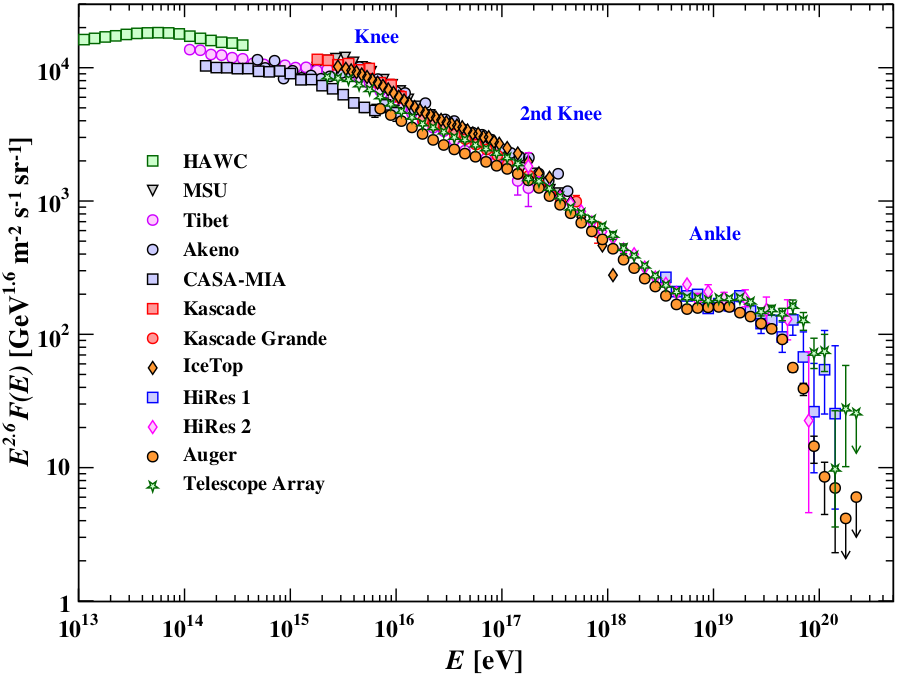
\includegraphics[width=0.8\linewidth]{Figs/CR_spectrum.png}
    \caption{Espectro de energía de los CR primarios. Los puntos con diferentes colores y geometrías indican las mediciones realizadas por experimentos directos o indirectos. Fuente \cite{PDG}}
    \label{fig:spectrum}
\end{figure}

%%%%%%  ORIGEN DE LOS RAYOS CÓSMICOS DE ANTES DEL TOBILLO Y DESPUÉS DEL TOBILLO.
%%%% Pierre Cristofari (The transition From Galactic to Extragalactic cosmic rays)
Existe evidencia que sugiere que los CR con energías inferiores a la “rodilla” del espectro energético, tienen un origen galáctico modulado principalmente por el viento solar. Esta afirmación se basa en la observación de los rayos gamma emitidos por el disco galáctico pues se espera que la interacción de los CR con el material interestelar genere una señal de rayos gamma mejorada, es decir, un incremento en la emisión (\cite{Cristofari_2023}).

Por otro lado, cuando la energía de los CR supera un cierto umbral, conocido como el “tobillo”, se tiene evidencia de un origen extragaláctico (\cite{augerextra}). Esta transición se produce porque los CR de alta energía no pueden confinarse dentro de la galaxia cuando su radio de Larmor, que es el radio de la trayectoria en espiral que una partícula cargada sigue en un campo magnético, es mayor que el tamaño típico del halo galáctico (\cite{spurio_2015}). 
%Se tiene evidencia de que los CR de energías inferiores a la "rodilla" del espectro energético son de origen galáctico. Esto se basa en la observación de los rayos gamma del disco galáctico de los que se espera la emisión de una señal de rayos gamma mejorada (un incremento en la emisión) debido a la interacción de los CR con el material interestelar (\cite{Cristofari_2023}). Sin embargo, cuando la energía de los CR supera cierto umbral, conocido como el "tobillo", la fuente es de origen extragaláctico (\cite{augerextra}). Esta transición se debe a que los CR de alta energía no pueden confinarse dentro de la galaxia cuando su radio de Larmor es mayor que el tamaño típico del halo galáctico.
\section{Propagación de CR a través de la heliósfera}

Independientemente de su procedencia, todas las partículas primarias tienen que atravesar los campos magnéticos terrestre y solar para entrar en la atmósfera y es su energía la que determinará si tienen o no una interacción significativa. El examen minucioso de la composición y estructura del magnetismo solar ha permitido avanzar sustancialmente en nuestra comprensión del Sol y la forma como este modula los CR que viajan por el espacio interestelar. 

Son varias las capas que componen este cuerpo celeste, y cada una de ellas es esencial para la creación y distribución de su energía. En concreto, el interior, que incluye el núcleo y la zona radiativa constituye aproximadamente el $70\%$ de su radio, y el $~30\%$ restante lo constituye la zona convectiva (\cite{Hanslmeier_2023}). En esta región, la temperatura no es lo suficientemente alta como para transferir energía a través de la radiación térmica. Por lo tanto, el plasma caliente cerca a la zona radiativa asciende hacia la superficie solar donde pierde energía. A medida que se enfría, el plasma desciende continuando el ciclo continuo de transporte. Este proceso de convección da lugar a un patrón celular en la superficie conocido como granulación solar (figura \ref{fig:sunspotNSO}) que a su vez, genera campos magnéticos a través de un mecanismo conocido como 'mecanismo de dínamo solar' (\cite{Sturrock_1986}).
%El resultado de la interacción y la influencia del sol sobre estas partículas dependen fuertemente de su energía. 
%El Sol debido a su proximidad y características, se ha convertido en un laboratorio esencial para la comprensión de la física estelar y es fundamental para la investigación en física del plasma y astrofísica (\cite{Rozelot_2006}). %%%%%ROZELOT
\begin{figure}
    \centering
    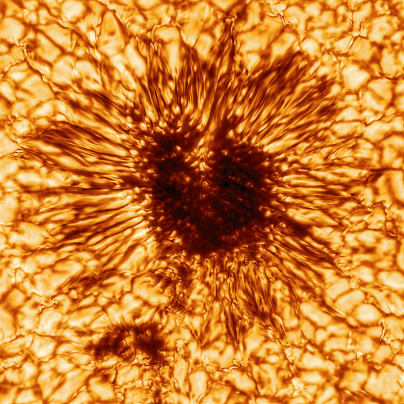
\includegraphics[width=0.6\linewidth]{Figs/sunspot_small.png}
    \caption{La cámara Inouye Solar Wave Front Correction (WFC) de la NSF capturó su primera imagen de una mancha solar el 28 de enero de 2020. La imagen revela un corte de la estructura tridimensional de la mancha solar, que se forma por la convergencia de campos magnéticos intensos y gas caliente que burbujea desde abajo. Aunque la imagen presenta una paleta de colores cálidos con tonos rojos y naranjas, fue tomada por el visor contextual de la Cámara de Campo Amplio del Telescopio Solar Inouye a una longitud de onda de 530 nanómetros, que corresponde a la parte amarillo verdosa del espectro visible. Crédito: NSO/AURA/NSF}
    \label{fig:sunspotNSO}
\end{figure}
La atmósfera del Sol, que incluye la fotósfera, la cromósfera y la corona, juega un papel crucial en su dinámica. Aunque estas capas representan una pequeña fracción del radio total ($0.43\%$), son el escenario de varios fenómenos que definen su actividad. La fotósfera, que es la capa que vemos desde la Tierra, tiene un grosor de aproximadamente 500 km y es donde se manifiestan las manchas solares, que son indicadores de su actividad magnética y su mecanismo de convección (figura \ref{fig:sunspotNSO}). La cromósfera, con un grosor de aproximadamente 2500 km, es el lugar donde ocurren las fulguraciones solares, que son explosiones de energía causadas por el reajuste de las líneas del campo magnético. 

Finalmente, la corona aunque se extiende mucho más allá de la cromósfera, es notablemente menos densa y es la fuente del viento solar compuesto principalmente por electrones y protones que se expanden hacia el exterior a velocidades de entre 300 y 800 kilómetros por segundo. Este flujo de partículas arrastra el campo magnético del Sol, formando una estructura helicoidal conocida como espiral de Parker (\cite{Rozelot_2006}) y extendiendo así a cientos de miles de kilómetros la influencia del Sol en una estructura denominada heliósfera. Se puede pensar la heliósfera como el escudo permanente ante los vientos interestelares (\cite{schrijver_2009}) ya que su existencia produce una dinámica compleja de campos magnéticos y partículas energéticas. De este modo, aunque la atmósfera representa solo una pequeña fracción del radio total, su influencia se extiende mucho más allá, teniendo repercusiones incluso en nuestra vida diaria en la Tierra.
%%%%%%%%%%% PUEDE SER UNA IMAGEN ACÁ PERO BUENO 

Las sondas espaciales dan la oportunidad de medir directamente parámetros físicos fundamentales del viento solar. Este no es un fluido estacionario: continuas fluctuaciones del campo magnético son producidas por movimientos turbulentos del gas, y escapan hacia el medio interplanetario. Discontinuidades en el campo magnético y ondas de choque se producen por la colisión de viento solar lento y viento solar rápido y por erupciones en la corona solar, eyecciones de masa coronal (CME) y fulguraciones. Las CMEs arrastran plasma solar a altas velocidades que se propagan a través del sistema solar, y pueden ser medidas cerca de la Tierra como ICME (Eyección de masa coronal interplanetaria). Cuando son suficientemente rápidas generan una onda de choque delante de ellas como se observa en la figura \ref{icme}. 

En la imagen podemos observar como la estructura magnética expulsada desde la corona (línea roja) perturba el campo magnético heliosférico (líneas azules). El viento solar no puede penetrar en la ICME, por lo que se comprime junto con el campo magnético, o se desvía alrededor de la ICME, como indican las dos flechas azules. La configuración de las líneas de campo cambia. En la interfaz entre la ICME y el viento solar circundante, el campo magnético se vuelve turbulento. En esta heliósfera perturbada, tanto los rayos cósmicos solares como los galácticos experimentan condiciones de propagación muy diferentes a las de la heliósfera en estado tranquilo (\cite{NMDB}).
\begin{figure}[H]
    \centering
    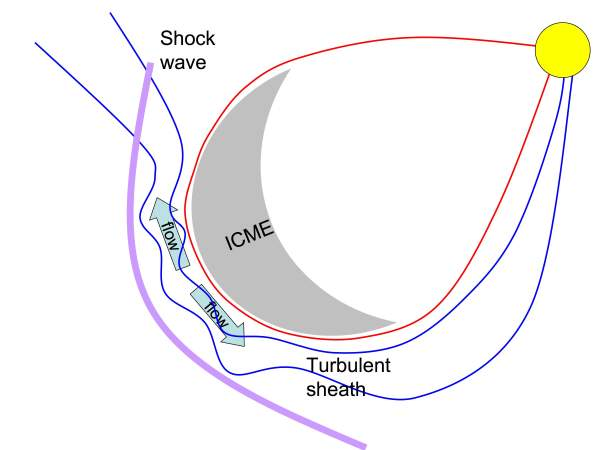
\includegraphics[width=0.5\linewidth]{Figs/Dessin_ICME_sm_0.jpg}
    \caption{Ilustración de la estructura magnética que se genera a partir de una CME desde la corona (línea roja) y perturba el campo magnético heliosférico representado por las líneas azules. El viento solar no puede penetrar en la ICME, por lo que se comprime junto con el campo magnético, o se desvía alrededor de la ICME, como indican las dos flechas azules. La alteración de la configuración de las lineas de campo en la región de propagación de la ICME le añaden turbulencia al campo magnético. Fuente \cite{NMDB}}
    \label{icme}
\end{figure}
Un ejemplo de esta dinámica se puede observar a través de la figura \ref{CME_2003} donde se muestran los registros de una fulguración intensa y una CME, que perturban considerablemente la heliósfera el 28 de octubre de 2003. Las cuatro imágenes fueron tomadas por diferentes instrumentos a bordo de la nave SOHO (ESA/NASA). Grupos de manchas (arriba a la izquierda) indican intensa actividad y complejas estructuras magnéticas en la superficie. En la mayor y más compleja de esas regiones aparecieron brillantes fulguraciones observadas por el telescopio de ultravioleta extremo EIT (esquina superior derecha). Además se observa una CME rápida y grande unos minutos más tarde por el coronógrafo LASCO (imágenes inferiores), propagándose por la corona a una velocidad de 1000 km/s.
\begin{figure}
    \centering
    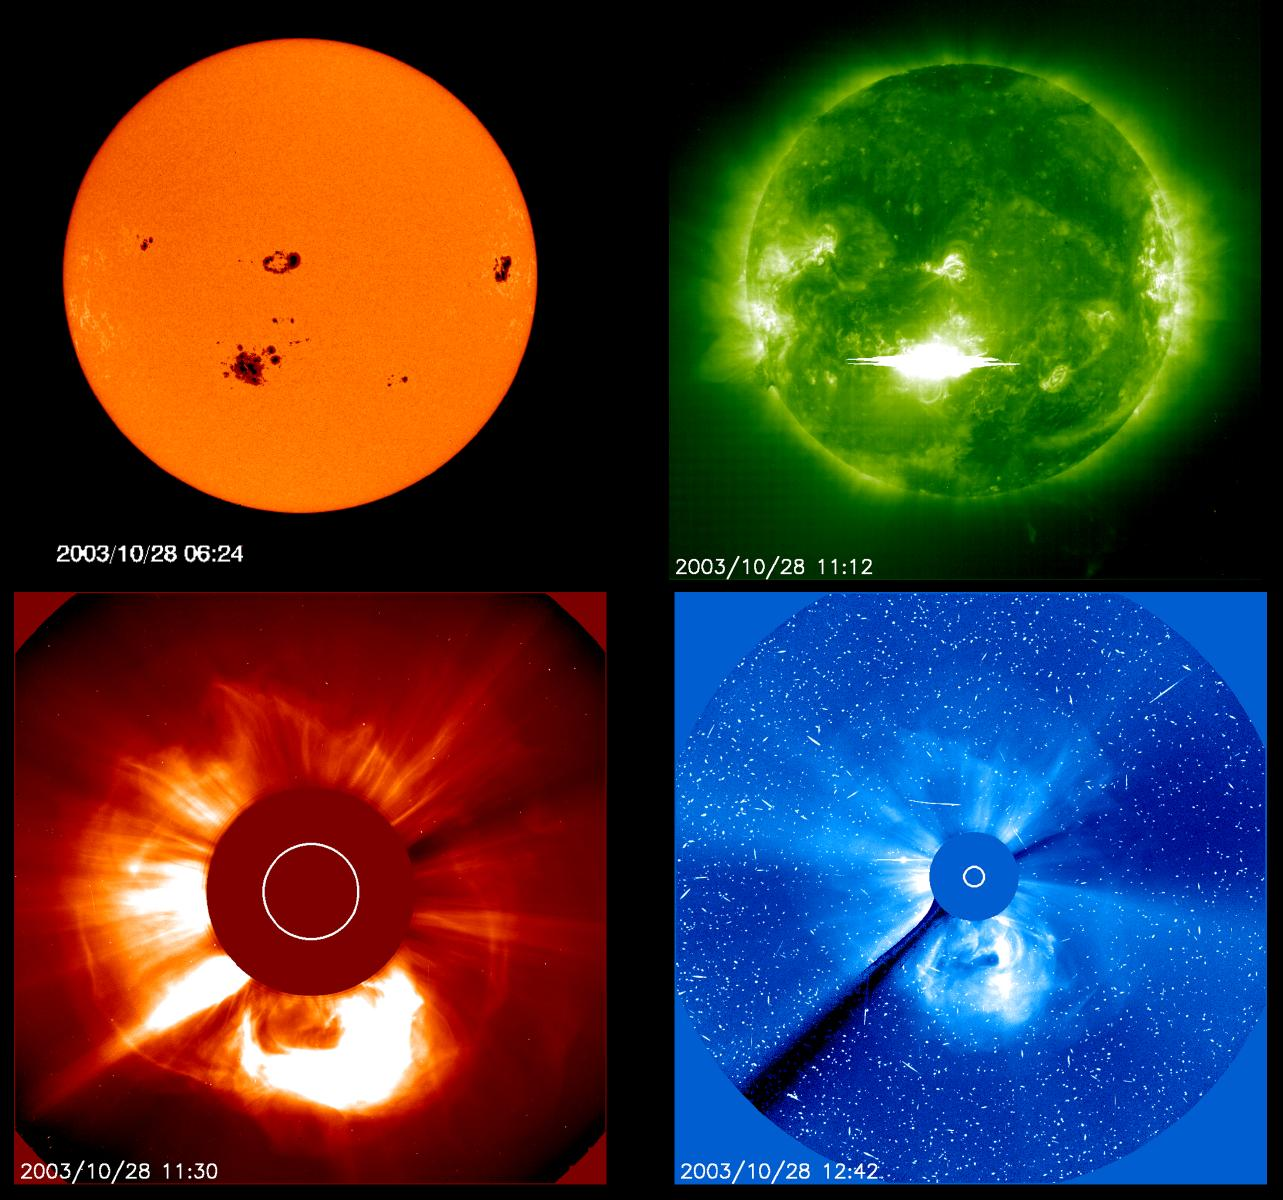
\includegraphics[width=0.5\linewidth]{Figs/flare_2003-10-28.jpg}
    \caption{Registros de una fulguración intensa y una CME, que perturban considerablemente la heliósfera el 28 de octubre de 2003. Las cuatro imágenes fueron tomadas por diferentes instrumentos a bordo de la nave SOHO (ESA/NASA). Grupos de manchas (arriba a la izquierda) indican intensa actividad y complejas estructuras magnéticas en la superficie. En la mayor y más compleja de esas regiones aparecieron brillantes fulguraciones observadas por el telescopio de ultravioleta extremo EIT (esquina superior derecha). Además se observa una CME rápida y grande unos minutos más tarde por el coronógrafo LASCO (imágenes inferiores), propagándose por la corona a una velocidad de 1000 km/s. Fuente SOHO/MDI, SOHO/EIT, SOHO/LASCO (ESA/NASA)}
    \label{CME_2003}
\end{figure}
Los rayos cósmicos galácticos (GCR) con energías altas $>10GeV$ poseen una trayectoria rectilínea  al propagarse por la heliósfera, ya que la fuerza de Lorentz que ejerce el campo magnético es despreciable en comparación con su momento lineal. Las partículas de energía moderada, de unos pocos $GeV$, tienen una trayectoria difusiva (\cite{gaisser_2016}). La difusión se produce por la presencia de irregularidades en el campo magnético del viento solar, que provocan cambios en la dirección e intensidad del campo a lo largo de la trayectoria de las partículas. Estos cambios se deben a la turbulencia del plasma, que genera fluctuaciones en el campo magnético a diferentes escalas espaciales y temporales (\cite{spurio_2015}). La difusión de los rayos cósmicos de energía moderada implica una pérdida de información sobre su dirección de origen y una modulación de su flujo en función del la actividad solar.
%%%%%%%%% NEW

Es importante destacar que la actividad solar varía en el tiempo. Uno de los periodos de mayor interés es el ciclo solar de 11 años. En este periodo, hay un notorio cambio en el número de manchas solares pudiéndose identificar un periodo de máxima formación y uno de mínima, que también está relacionado con cambios bruscos en el viento solar y el campo magnético interplanetario como se observa en la figura \ref{fig:100ysn}. La modulación del flujo de rayos cósmicos de energía moderada puede verse afectada por estas variaciones de la actividad solar a través de su dispersión. Sin embargo, los GCR también presentan variaciones de menor amplitud y duración, relacionadas con la rotación solar de 27 días y con la localización de las regiones activas en el Sol. Estas variaciones se deben a que el viento solar y el campo magnético interplanetario no son homogéneos ni isotrópicos, sino que dependen de la latitud y la longitud solar. Así, los GCR experimentan cambios en su flujo, su espectro de energía y su anisotropía, que es la distribución angular de su intensidad.

Otro aspecto importante del ciclo solar es que cada 11 años el campo magnético solar invierte su polaridad, lo que implica que el ciclo completo es de 22 años. Esto afecta a la propagación de los GCR en la heliósfera, ya que el campo magnético interplanetario tiene una configuración diferente según la polaridad del campo magnético solar. De esta forma, el flujo de GCR tiene una forma distinta en dos ciclos solares consecutivos. En uno, el flujo tiene un pico pronunciado, con un máximo claro, mientras que en el otro, el flujo tiene una forma más plana, con un máximo menos definido. No obstante, las escalas superiores al ciclo solar de 11 años quedan por fuera de los alcances de este trabajo.
\begin{figure}
    \centering
    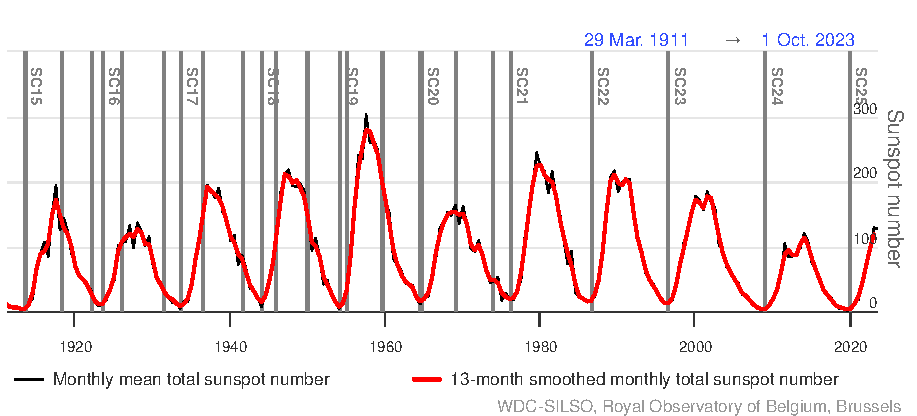
\includegraphics[width=0.8\linewidth]{Figs/sunspots.pdf}
    \caption{Ciclos solares en los últimos 100 años observados a partir del número de manchas solares. Fuente WDC-SILSO, Royal Observatory of Belgium, Brussels}
    \label{fig:100ysn}
\end{figure}

\section{Propagación de CR a través del Campo Geomagnético}

La Tierra está rodeada por un campo magnético casi dipolar generado por las corrientes eléctricas de su núcleo. A esta región del espacio donde el campo magnético terrestre es predominante sobre el campo magnético interplanetario se llama magnetosfera y tiene una forma asimétrica, como se muestra en la figura \ref{magnetosfera}. 

El viento solar interactúa con el campo magnético comprimiéndolo en la dirección del Sol y lo estira en la dirección opuesta, creando una cola magnética (figura \ref{magnetosfera}).  De la misma forma, la interacción de los RC primarios con el campo geomagnético terrestre también modula su intensidad a nivel del suelo. El campo geomagnético desvía las trayectorias de las partículas primarias según su rigidez $R$, que es la relación entre su cantidad de movimiento $p$ y su carga $q$. 
\begin{equation}
    R=\frac{p}{q}=r_{L}B.
\end{equation}
Donde $r_L$ representa el radio de Larmor, parámetro usado para determinar la capacidad que tiene una partícula de penetrar el campo magnético en una ubicación específica. En un campo geomagnético dipolar como el de la Tierra, el momento mínimo por carga que una partícula debe tener en una ubicación determinada se puede describir con la rigidez de corte $R_C$:
\begin{equation}
    R_C=\kappa\frac{1}{L^{\alpha}}
    = \frac{M cos^{4}\lambda}{4r^{2}},
\end{equation}
donde $L$ es el parámetro McIlwain, que denota la distancia a la que una línea de campo magnético cruza el plano ecuatorial, $M$ representa el momento dipolar, $r$ la distancia desde el centro del dipolo (en unidades de radios terrestres), $\lambda$ la latitud geográfica, y las constantes $\kappa$ y $\alpha$ valen $\approx 14.823GV$ y  $2,0311$ respectivamente. Esta ecuación es válida solo para latitudes altas e ignora la geometría del campo. Además, la estructura del campo magnético de la Tierra es mucho más intrincada que la de un dipolo simple. Por tanto, para calcular RC en cualquier campo magnético se deben realizar cálculos numéricos.

\begin{figure}
    \centering
    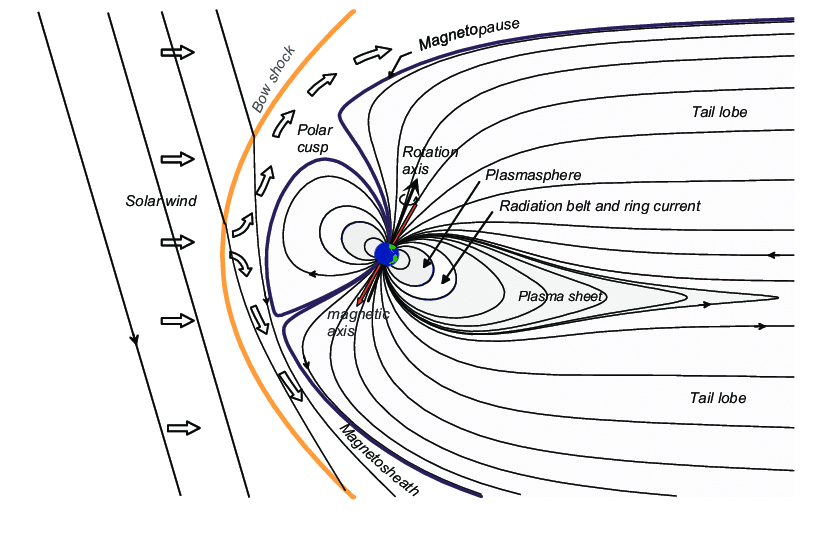
\includegraphics[width=0.7\linewidth]{Figs/Schematic-representation-of-the-near-Earths-magnetosphere.png}
    \caption{Representación esquemática del campo geomagnético terrestre. Fuente \cite{tenerani_2012}}
    \label{magnetosfera}
\end{figure}
%%%% ESTO VA ABAJOOOOOOOOOOOOOOO
\textbf{Decrecimientos Forbush (FD)}: Son disminuciones breves de la intensidad de los GCR seguidas de una lenta recuperación, que suele durar varios días (\cite{forbush_1954}). Inicialmente se atribuyeron a las erupciones solares, pero más tarde se descubrió que estaban causados por CME (\cite{lingri_2016}). Este fenómeno corresponde a los eventos de rayos cósmicos más importantes registrados en los monitores de neutrones terrestres y tienen características diferentes en relación con los parámetros de actividad solar durante las distintas fases de los ciclos solares. La amplitud de las disminuciones de intensidad de los rayos cósmicos que miden estos monitores varía con la diferente rigidez de corte de cada estación alcanzando registros de hasta un $25\%$ (\cite{cane2000}).

 Los FD pueden clasificarse en dos tipos: no recurrentes y recurrentes. Los no recurrentes tienen un inicio repentino y están asociadas a perturbaciones transitorias del viento solar. Tienen perfiles asimétricos y se ven afectados por el área, la velocidad y la fuerza del campo magnético irregular de las CME (\cite{cane2000}, \cite{lingri_2016}). Contrariamente los decrecimientos recurrentes tienen un inicio gradual, un perfil simétrico y están bien asociadas con corrientes de viento solar de alta velocidad corrotantes que son más frecuentes en los periodos de alta actividad solar (\cite{lingri_2016}, \cite{kallaya_2021},\cite{wang_2023}). La figura \ref{forbush}  muestra un FD registrado en mayo de 2005 por el observatorio Pierre Auger y el monitor de neutrones de Los Cerrillos (Chile). 
\begin{figure}[H]
    \centering
    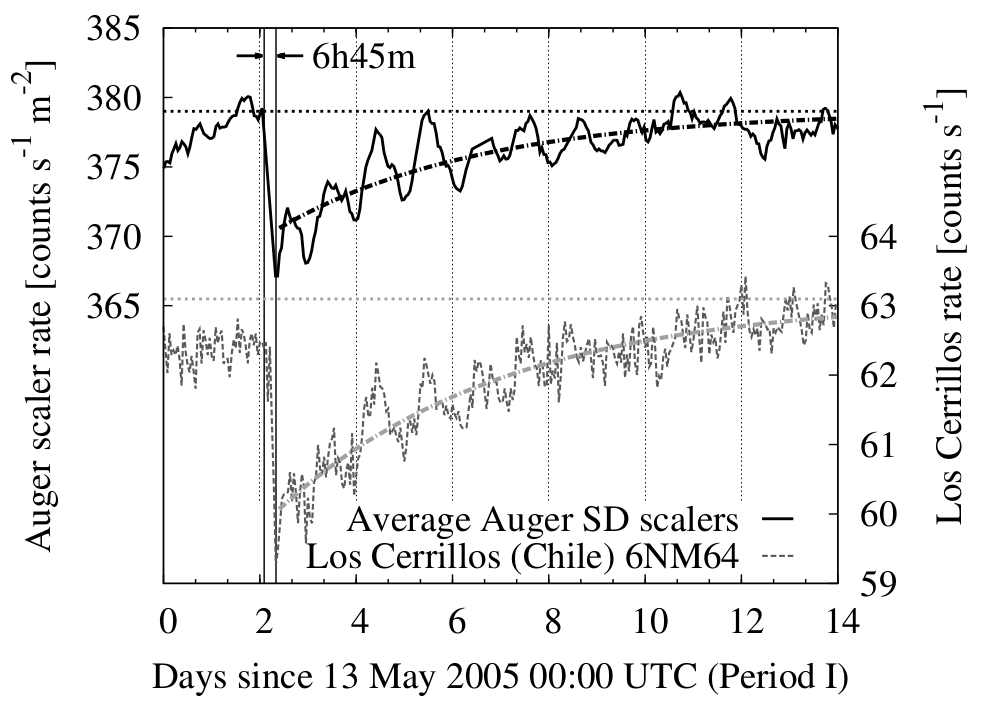
\includegraphics[width=0.6\linewidth]{Figs/mauro_forbush.png}
    \caption{Perfil de un Decrecimiento Forbush ocurrido el 13 de mayo del 2005. Se observa la comparación del evento medido por el Observatorio Pierre Auger en contraste a la señal obtenida con el monitor de neutrones de Los Cerritos en Chile, escogido por la similitud de las rigideces de corte geomagnético. Fuente \cite{asorey_2012}}
    \label{forbush}
\end{figure}
En el caso de los FD no recurrentes, la disminución del flujo de rayos cósmicos se debe al efecto de apantallamiento que produce la estructura magnética de la ICME y la onda de choque que la acompaña, tal como se representa en la figura \ref{icme} (\cite{papaioannou_2020}). El campo magnético de la ICME es más intenso y turbulento que el del viento solar, lo que dispezrsa más a los rayos cósmicos y los desvía de su trayectoria original (\cite{belov_2009}). Además, la onda de choque de la ICME comprime el plasma y el campo magnético, lo que crea una barrera que dificulta el paso de los rayos cósmicos. Estos efectos son más notorios para las partículas de menor energía, que son más sensibles a la fuerza de Lorentz que ejerce el campo magnético. Así, los rayos cósmicos que atraviesan una ICME sufren una modulación de su flujo, su espectro de energía y su anisotropía.

\section{Propagación de CR a través de la atmósfera terrestre}

Cuando los CR primarios llegan a la atmósfera terrestre, chocan con los átomos del aire y producen una lluvia de partículas EAS que tienen menos energía que el primario. Algunas de estas partículas pueden decaer o interactuar nuevamente, generando una reacción en cadena (\cite{gaisser1990}) que se detiene cuando la energía del primario se disipa o se alcanza el nivel del suelo.

Durante el desarrollo de una EAS las partículas recorren una cierta cantidad de materia a medida que atraviesan la atmósfera. Este parámetro comúnmente llamado profundidad atmosférica $X(h)$, depende de la altura $h$ sobre el nivel del mar y de la densidad del aire $\rho(h)$.  
\begin{equation}
X_{v}= \int_{h}^{\infty} \rho (h') dh'.
\label{eq:eq2}
\end{equation}
Las interacciones producidas a lo largo del desarrollo de la cascada a través de una cierta cantidad de materia $X(h)$ permiten identificar tres componentes principales: una electromagnética, que está conformada por electrones, positrones y fotones; otra hadrónica, constituida de piones, kaones y bariones, y una componente muónica, generada por el decaimiento de piones y kaones cargados. La figura \ref{fig:fig3} ilustra los procesos de interacción mostrados anteriormente y cómo éstos generan cada una de las componentes. Como se observa en la imagen, la producción de partículas secundarias está mediada por interacciones electromagnéticas y hadrónicas que describiremos con un poco más de detalle a continuación.

\begin{figure}[htb!]
\centering
    \begin{center}
        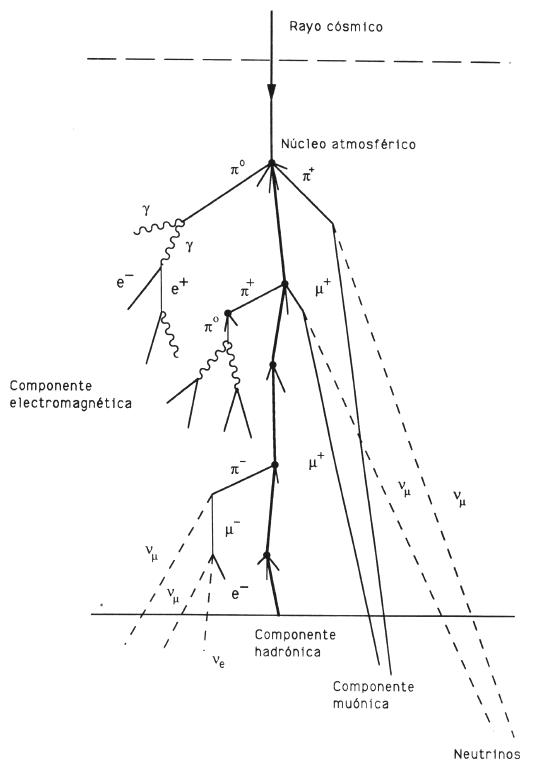
\includegraphics[width=0.5\textwidth]{Figs/componentes_cas.jpg}
    \end{center}{}
    \caption[Esquema del desarrollo de una EAS iniciada por un hadrón.]{Esquema del desarrollo más probable de una EAS iniciada por un hadrón \cite{mauro:tesis}. En la figura se observa el decaimiento del hadrón en piones cargados y neutros, y estos a su vez, al decaer, generan fotones, electrones y muones. Se identifican tres componentes: electromagnética, muónica y hadrónica.}
    \label{fig:fig3}
\end{figure}

\subsection{Interacciones electromagnéticas}
Están presentes cuando el primario incidente es un fotón o un electrón. Estas partículas pueden crear o emitir otras partículas del mismo tipo al interactuar con los átomos del aire. Por ejemplo, los fotones pueden crear pares de electrones y positrones, y estos pueden emitir más fotones al frenarse (bremsstranhlung). Este proceso se detiene cuando los fotones tienen una energía de $1.02 MeV$. En el caso de un núcleo de aire con carga $Z$ y número atómico $A$, los procesos de producción son (\cite{heitler}):
 %para quienes el principal canales de interacción son la producción de pares y radiación de frenado. E
\begin{equation}
\begin{split}
&Bremsstrahlung\quad e \quad \xrightarrow{Y^{A}_{Z}} \quad e\gamma ,  \quad y \\
&Pares \quad \gamma \xrightarrow{Y^{A}_{Z}} \quad e^{+}e^{-}. \\
\end{split}
\end{equation} 
Otros procesos electromagnéticos que influyen en esta pérdida de energía y deben ser considerados son:

\textbf{La pérdida de energía por Ionización} de una partícula cargada que atraviesa la materia con un espesor $\lambda$ que es descrita por la ecuación de Bethe-Bloch:
\begin{equation}
dE_{i} = \frac{\lambda \gamma^{2}z^{2}}{\gamma^{2}-1}\kappa_{1}(ln(\gamma^{2}-1)- \beta^{2}+\kappa_{2}).
\label{eq:eq20}
\end{equation}

Donde $\beta = v/c $ es la velocidad de la partícula en unidades de la velocidad de la luz, $\gamma$ es el factor de Lorentz, $z$ es la carga de la partícula ionizada en unidades de $e$. Las dos constantes $\kappa_{1}= 0.153287$ $ MeV g^{-1}$ y $\kappa_{2}= 9.386417 $ $MeV g^{-1}$ son los valores correspondientes para el aire (\cite{Heck1998}). Esta expresión es usada para calcular la perdida por energía de ionización a través de la trayectoria de la partícula. Por ejemplo, la pérdida de energía de muones como función de su energía está representada en la figura \ref{fig:fig4}.
\begin{figure}[htb!]
\centering
        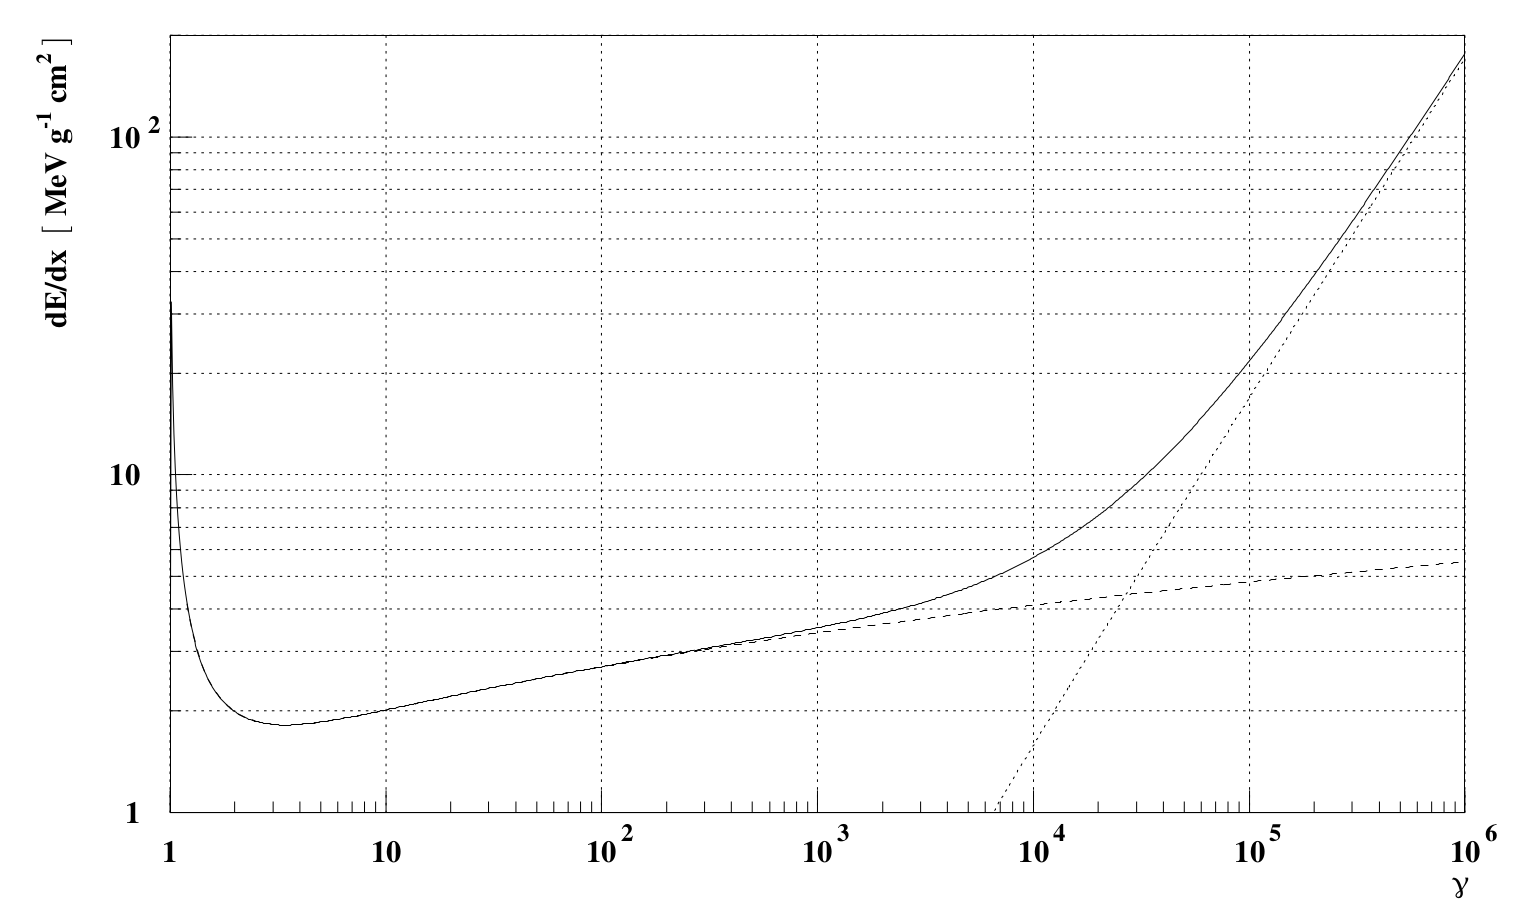
\includegraphics[width=0.7\textwidth]{Figs/Bethe_Muons.png}
        \caption[Ecuación de Bethe-Bloch para los muones.]{Pérdida de energía de Muones en el aire como función del factor de Lorentz . Están indicadas las contribuciones de la ionización (línea seccionada) y la producción de pares (línea punteada). Fuente: \cite{Heck1998}}
        \label{fig:fig4}
\end{figure}

La \textbf{Dispersión múltiple de Coulomb} que ocurre cuando las partículas cargadas son dispersadas por el campo eléctrico Coulombiano de los núcleos de aire. Allí la dirección de propagación es alterada pero no cambia la energía de la partícula. La distribución angular de esta dispersión es descrita por la teoría de Moliére (\cite{Heck1998}).  

\subsection{Interacciones hadrónicas}
%%%%% NEW
Las interacciones hadrónicas son un componente fundamental en el estudio de las EAS. Aunque la cromodinámica cuántica proporciona una base sólida para entender las interacciones fuertes, los procesos con múltiples partículas producidas en las interacciones hadrónicas aún no pueden ser calculados con precisión. Para superar esta limitación, se han desarrollado modelos que hacen suposiciones adicionales y utilizan parametrizaciones fenomenológicas y empíricas (\cite{Allen}). Estos modelos son esenciales para interpretar las EAS y deben estar optimizados para un amplio rango de energías. Además, es crucial que se actualicen constantemente a medida que se obtienen más datos de los aceleradores o de grandes instrumentos como el Observatorio Pierre Auger \cite{andrada_2021}. Las interacciones hadrónicas generan piones cargados y neutros ($\pi^{-},\pi^{+},\pi^{0}$), así como kaones, que tienen una tendencia mayor a decaer que a interactuar. Los canales de decaimiento más probables para estas partículas son los siguientes:
\begin{align*}
\pi^{0} &\rightarrow \gamma\gamma \quad [{98.823 \pm 0.034}{\%}], \\
\pi^{0} &\rightarrow e^{+}e^{-} \gamma \quad [{1.174 \pm 0.035}{\%}], \\
\pi^{+} &\rightarrow \mu^{+}\nu_{\mu} \quad [{99.98 \pm 0.00004}{\%}], \\
\pi^{-} &\rightarrow \mu^{-}\nu_{\mu} \quad [{99.98 \pm 0.00004}{\%}], \\
K^{+} &\rightarrow \mu^{+}\nu_{\mu} \quad [{63.56 \pm 0.11}{\%}], \\
K^{+} &\rightarrow \pi^{0}e^{+}\nu_{e} \quad [{5.07 \pm 0.004}{\%}], \\
K^{+} &\rightarrow \pi^{+}\pi^{0} \quad [{20.67 \pm 0.08}{\%}] \quad y \\
K^{+} &\rightarrow \pi^{+}\pi^{+}\pi^{-} \quad [{5.583 \pm 0.024}{\%}].
\end{align*}
Estos procesos contribuyen a la componente electromagnética y muónica de las EAS. Más específicamente, la componente muónica en las EAS es de particular interés debido a las propiedades relativistas de los muones y su larga vida media. Esta componente ofrece una visión directa de las primeras interacciones hadrónicas y las propiedades del hadrón inicial. Los muones de alta energía desencadenan sub-cascadas electromagnéticas y hadrónicas en la lluvia a través de interacciones tipo:
\begin{align}
\mu^{\pm} \quad &\xrightarrow{Y^{A}_{Z}} \quad \mu^{\pm}e^{+}e^{-}, \\
\mu^{\pm} \quad &\xrightarrow{Y^{A}_{Z}} \quad \mu^{\pm} + \text{hadrones}.
\end{align}